\chapter{Functional Function Fun}
\label{chap:Functions}

Mathematicians are \emph{really} fond of definitions. Often, mathematicians will spend large parts of their day worrying about the precise definition of some concept, whereas a scientist or an engineer may just take it on intuition. Sometimes in this book, we'll take the route of the engineer, and just go with what makes sense. However, if we want to get started on the right foot, we'll need to make sure that we know exactly what we mean by the word ``function''.

\section{What is a function?}
In pre-calculus, you may have discussed a function as an ``input-output machine'', meaning that it takes one number in, and puts one number out. A slightly better way to put it is to say that a function is a strict rule for associating an input number with an input number. By \emph{strict}, we mean that it is totally unambiguous; there should be no room for guessing about the interpretation of a function. For example,

\[f(x) = \frac{x^2}{6}\]\\

is a strict rule. For any number $x$ we can think of, it is absolutely clear how to calculate $f(x)$: we multiply $x$ by itself, then divide that number by $6$. On the other hand,

\[g(x) = \frac{x^2}{\text{Number of seconds since the author's last Peanut Butter sandwich}}\]\\

is quite ambiguous; do we count the seconds since the author finished his sandwich, or the number since he began? Further, suppose the author was interrupted from his sandwich by the sudden arrival of an infinite gaggle of Canadian Geese, each requesting an equal-sized crumb. Clearly it would be quite impossible to interpret this expression without opening a hole for philosophers to crawl in and shout at us about the follies of loose reasoning. No, better to wash our hands of it and stick to polynomials for the time being. 

\section{Polynomials}
In this book, we shall limit our discussion of functions to polynomials of real numbers, such as $x^2$, $2x^3 + 5x^2$, and even $\pi x^3 + 0.001x + 6$. We will not (at first) consider any exponential functions ($e^x$), nor any trigonometric functions($\sin(x)$, $\cos(x)$, etc\ldots), nor any other form of high-brow transcendental lavishness (hyperbolic functions, Bessel functions, respiratory functions\ldots). In general, polynomials look like this:

\[f(x) = a_0 x^0 + a_1 x^1 + a_2 x^2 + \cdots + a_n x^n\]\\

Where each of the $a_i$ are just whatever real numbers we choose. Every different choice of the $a_i$'s gives us a different polynomial. For example, let's pick two polynomials of degree\footnote{The \emph{degree} of a polynomial is the highest number to which $x$ is raised: $x^5 + x^4$ is a fifth-degree polynomial, $x^2 + x + 1$ is a second-degree polynomial. If we're being general, we say that $x^n + x^{n-1} + \cdots + x^1$ is an $n$-th degree polynomial} 1: 

\[p_1(x) = 5 x^0 + 4 x^1\]
\[p_2(x) = 3 x^0 + 4 x^1\]\\

These are different polynomials, which should be obvious enough. Given the same input, say $x=0$, they will give different output values: $p_1(0)$ will equal 5, wheras $p_2(0)$ will equal 14\footnote{Are you working these by hand as we go along? Because $p_2(0)$ is definitely not 14\ldots}. If we plot these two functions, we will see that while they may overlap in some places, mostly they are different. 

Fortunately, we do not have to check polynomials by hand or plot them to see if they are different: polynomials can be entirely characterized by their \emph{coefficients} -- that is, the specific values of $a_0$, $a_1$, etc. That means we could represent $p_1(x)$ as $(5,4)$ and $p_2(x)$ as $(3,4)$, which we can then treat as points in the plane.

In fact, it is a central idea in this book that there is a connection between points in the plane and polynomials of degree 1. The same connection also holds between polynomials of degree 2 (such as $12x^2 - 100x^1 + 17x^0$) and points in a three-dimensional space, like $(12,-100,17)$. This connection allows us to use a neat tool from geometry, namely \emph{linear maps}, to study properties of polynomials having to do with rates of change. That's actually what Calculus is all about.

\section{Functions in Python}
The tutorials in this book use the IPython \cite{PER-GRA:2007} package. Please take a moment to install IPython on your computer so that you can follow along. Install instructions are available online: \url{http://ipython.org/install.html}.

Let's take a look at a simple polynomial function in Python:

\begin{python}
def f(x):
	return x + 2
\end{python}

This code does nothing more than to declare that \pyth{f} is the function $f(x) = x + 2$. In the same fashion, if we wanted to define the function $g(x) = x^2 + 3$ in Python, we could do that just as easily:

\begin{python}
def g(x):
	return x*x + 3
\end{python}

Let's talk about what each statement does in a little more detail, so that these code examples become a bit clearer. 

Do you remember earlier when we discussed how much mathematicians love definitions? Well, computers are equally obsessed with definitions, so if we want to get anything done in Python, we will need to begin by \emph{defining} what we are talking about. We can introduce a new function definition with the \pyth{def} keyword. In fact, the Python expression ``\pyth{def g(x):}" simply means ``define a new function \pyth{g} that takes a single input variable \pyth{x}".

The lines below the ``\pyth{def g(x):}" statement are called the \emph{body} of the function, and they tell Python what the function is all about. In this case, we want to calculate the value $x^2 + 3$, so we tell Python to multiply $x$ by itself (\pyth{x*x}) and then add 3. The \pyth{return} keyword simply tells python "what comes after is the \emph{output} of this function". Once the \pyth{return} statement has been called, the function will end.

One more note about the bodies of functions\ldots they must always be indented by 1 tab relative to the \pyth{def} statement. This is because Python assumes that the function body extends down until the first line that isn't indented. So, for example, if you were to omit the tab and write the following code:

\begin{python}
def h(x):
return x*x + 3
\end{python}
you would get the following error at runtime\footnote{The phrase \emph{at runtime} is programmer speak for ``while your code is running". Using this phrase will make you sound savvy and professional, like you \emph{know what you're on about}.}:

\begin{python}
  File "<mycode.py>", line 2
    return x*x + 2
         ^
IndentationError: expected an indented block
\end{python}

\section{Python Polynomial Package}
To facilitate our work with polynomials, the author has kindly provided\footnote{You're welcome.} a \emph{package} that contains some pre-rinsed, ready-to-eat Python algorithms for dealing with polynomial functions. To use this package, we first need to \emph{import} it, so that the definitions it contains will be available to use in our IPython session:

\begin{python}
from polynomial import *
\end{python}

Simple as that. Before we move on, let's ask what that phrase really means. The first clause, \pyth{from polynomial}, means ``I'm referring to a file called \pyth{polynomial.py}, which may be in the current directory, or somewhere else in the \emph{library path}\footnote{More on paths later; for now, just note that the library path is a set of folders that contain other python packages. These were created for you as part of the IPython install. You will not have to worry about the details of paths during the course of this book}". The second clause, \pyth{import *}, means ``grab every definition you see". So I guess in English it would be ``Grab every definition you see from the polynomial.py file".

Now that we've imported this package, we can create new polynomial functions just by specifying their coefficients. Remember earlier how we said that their is a relationship between polynomials of degree 1 and points in the plane? Well, let's consider the points $P = (5,4)$ and $Q = (3,4)$:

\begin{figure}[t]
	\centering
	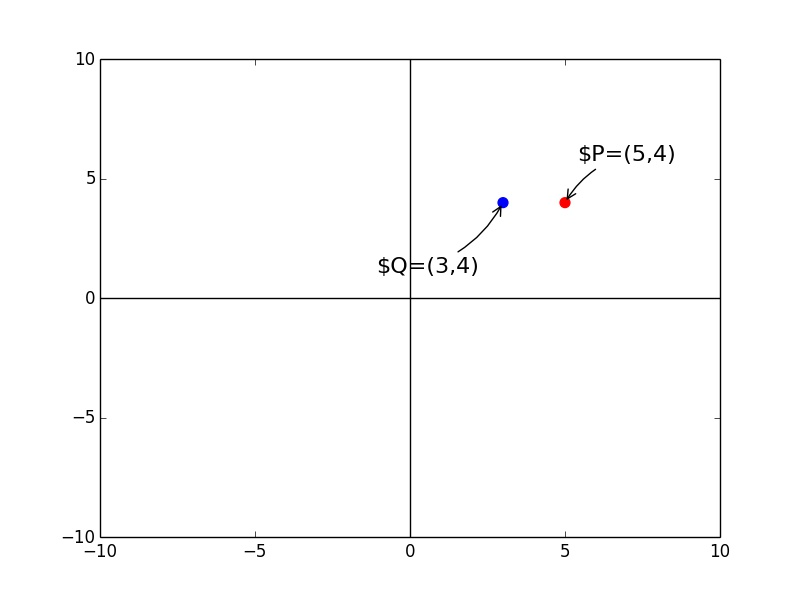
\includegraphics[scale=0.25]{BookSource/Chapters/p_and_q_hanging_out.jpg}
	\caption{$Q$ and $P$. Just hanging out in the plane.}
	\label{fig:p_and_q_hanging_out}
\end{figure}
and two corresponding polynomials, $f_P(x) = 5x + 4$ and $f_Q(x) = 3x + 4$:

\begin{python}
	fP = Polynomial([5,4])
	fQ = Polynomial([3,4])
\end{python}

Now, so far, this connection between points and polynomials might be no more than a silly notational coincidence. However, let us consider what it means to \emph{add} two points; if there is a relationship between adding points and adding polynomials, we could be convinced that this relationship is deeper than mere coincidence.

So, adding points\ldots First, let's talk about the definition of a point. When we say $Q = (3,4)$, what we mean is ``Starting from the origin\footnote{That is, the point $(0,0)$}, move 3 units along the $x$-axis, and then 4 units along the $y$-axis: here lies the point $Q$". 

\section{Exercises}
\begin{ExerciseList}
	\Exercise{Follow the instructions given at \url{http://ipython.org/install.html} to install IPython on your workstation. If you are using a shared workstation, such as a computer in the library or university commons, ask your professor to harass the campus IT department until they IPython for you (again, using the above instructions). Should the IT department intransigently refuse to assist you, engage in an act of non-violent civil disobedience such as: staging a teach-in in front of the Help Desk, railing against their fascist behavior in pastel sidewalk chalk, or perhaps asking the custodial union to \ldots hold off a while on their next IT department trash pickup. Write an essay about your experience.}
	\Exercise{How can you tell Python to import the module \pyth{polynomial.py}?}
	
	\Exercise{Given two polynomials $f$ and $g$, does it make sense that $f(x) + g(x)$ should always be the same as $(f + g)(x)$? That is, if we evaluate the functions first and then add their sum, will we get a different answer than if we add the polynomials first (i.e. create a new polynomial by adding their coefficients) and then evaluate the new polynomial?}
	\Exercise{Explain why the \emph{bodies} of functions must always be indented.}
	\Exercise{Describe in words what each line of the following Python function does:}
\begin{python}
def distance(x1,y1,x2,y2):
	deltaX = (x1 - x2)
	deltaY = (y1 - y2)
	return pow(pow(deltaX,2) + pow(deltaY,2),0.5)
\end{python}
\end{ExerciseList}